\documentclass[conference]{IEEEtran}
\IEEEoverridecommandlockouts
% The preceding line is only needed to identify funding in the first footnote. If that is unneeded, please comment it out.
\usepackage{cite}
\usepackage{amsmath,amssymb,amsfonts}
\usepackage{algorithmic}
\usepackage{graphicx}
\usepackage{textcomp}
\usepackage{xcolor}
\def\BibTeX{{\rm B\kern-.05em{\sc i\kern-.025em b}\kern-.08em
    T\kern-.1667em\lower.7ex\hbox{E}\kern-.125emX}}
\begin{document}

\title{ Low-Supply Voltage Sensor with an Optical Indicator: Design, Construction, and Analysis}

\author{\IEEEauthorblockN{1\textsuperscript{st} Miguel Villa Floran}
\IEEEauthorblockA{\textit{Computer Engineering Department} \\
\textit{California Polytechnic State University, San Luis Obispo}\\
San Luis Obispo, United States of America \\
miguel.villafloran@gmail.com}
}

\maketitle

\begin{abstract}
This experiment focuses on the design, construction, and analysis of a low-supply voltage sensor-indicator circuit employing a Zener diode based voltage limiter, linear voltage divider, and LED-based optical indicator. Key components include a 4.3 V Zener diode, TLC3702 voltage comparator IC, and a multi-turn potentiometer. The circuit utilizes a linear voltage divider and Zener diode to monitor supply voltage, activating an LED when the voltage drops below a specified threshold. The experiment providing valuable insights into the functionality and performance of the designed circuit

\end{abstract}

\begin{IEEEkeywords}
Zener diode, voltage comparator, LED, linear voltage divider, voltage limiter, potentiometer
\end{IEEEkeywords}

\section{Introduction}

\subsection{Voltage Comparator}

The voltage comparator is a device that specializes in comparing the voltages of two incoming signals and producing a high or low output voltage to indicate which is larger. If the the voltage across the positive terminal $V_{in+}$ is greater than the voltage across the negative terminal $V_{in-}$, the voltage comparator generates a logical high output voltage $V_{DD}$. Otherwise, a logical low output voltage $V_{SS}$ is produced \cite{week6}.

The voltage comparator is utilized in this design to indicate whether the voltage supply drops below a specified threshold, which for our intents and purposes is 8 V.

\subsection{Voltage Limiting Zener Diode}
The Zener Diode exhibits similar behaviors and properties as the standard PN junction diode. However, Zener diodes are also designed to have a well-defined and sharp reverse breakdown voltage, also referred to as the Zener voltage ($V_z$). When a Zener diode connected across a circuit in reverse bias reaches its Zener voltage, it maintains its Zener voltage and behaves as a closed circuit regardless of current fluctuations and changes in voltage. It is safe to use a Zener Diode in breakdown so long as the power it dissipates is below its maximum power rating \cite{week7}.

\begin{figure}[htbp]
\centerline{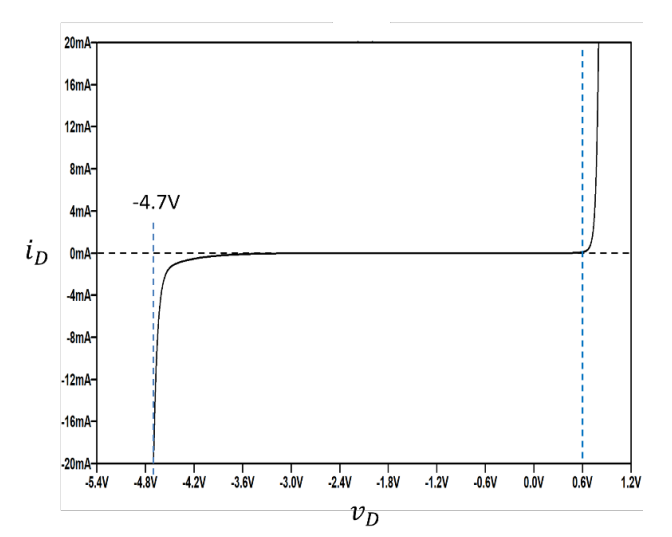
\includegraphics{./images/vi-characteristics.png}}
\caption{VI Characteristic of the 4.3V Zener Diode. \cite{week7}}
\label{fig}
\end{figure}

The reverse breakdown properties of a Zener Diode are leveraged to create voltage limiters for regulating the voltage across sensitive components or to provide constant reference voltages \cite{week7}. This is done by connecting a resistor, which limits the current coming into the diode, in series to the Zener Diode, which is connected in parallel to the load. In this design, the Zener Diode provides a constant voltage across the negative terminal of the comparator \eqref{eq_1}.

\begin{equation}
V_- \approx V_Z\label{eq_1}
\end{equation}

\subsection{Multi-Turn Potentiometer}

A multi-turn rotary potentiometer is a voltage divider whose resistance ratio can be adjusted, allowing for variable control of the output voltage in electronic circuits. The relationship of a typical potentiometer-based voltage divider can be found in \eqref{eq_2}. This adjustable resistance is utilized in this circuit so that the positive terminal's voltage is configured to be equivalent to the negative terminal's voltage when the supply voltage equals the threshold voltage. This ensure comparator is tripped at the threshold voltage. The values of the potentiometer can also be found mathematically by using \eqref{eq_3}, but in our case was found experimentally.

\begin{equation}
V_{out} = \frac{R_a}{R_a + R_b} V_{in}\label{eq_2}
\end{equation}

\begin{equation}
V_{DD(trip)} = (1 + \frac{R_b}{R_a})V_{Z}\label{eq_3}
\end{equation}

\subsection{LED Optical Indicator}

The light-emitting diode (LED) indicator serves as a visual cue, activating when the supply voltage falls below the predetermined threshold. The LED is reverse-biased relative to the output of the comparator and its cathode is connected to the supply voltage to ensure it only lights up when the supply voltage drops below the threshold voltage. When the supply voltage is above the threshold voltage, the comparator outputs the supply voltage, and the LED does not activate as there is no potential difference across it. When the supply voltage is below the threshold voltage, the comparator outputs 0 V, and the LED activates as there is a potential difference across it. To ensure the LED does not burn out, a resistor is added to limit current coming into the LED. This resistance is found by using \eqref{eq_4}.

\begin{equation}
R_{LED} \approx \frac{V_{DD(trip)} - V_{LED}}{I_{LED}}\label{eq_4}
\end{equation}

\section{Sensor Construction, Testing, and Data Collection}

This experiment required a single circuit to be assembled and tested in four phases as shown in figures \ref{circuit1}, \ref{circuit2},  \ref{circuit3}, and \ref{circuit4} to ensure its proper functionality and performance. For all circuits, the comparator was implemented using a TLC3702 voltage comparator IC, the optical indicator was implemented using a WP7113ID 617nm Red LED, the voltage limiter was implemented using a 1N5229BTR 4.3 V Zener Diode, and the voltage divider was implemented using a 5.00E-250 multi-turn potentiometer \cite{parts}.

\subsection{Testing the Zener-based Voltage Limiter}

The first phase involved the assembly of the Zener-based voltage limiter, as depicted in Fig. \ref{circuit1}.

\begin{figure}[htbp]
\centerline{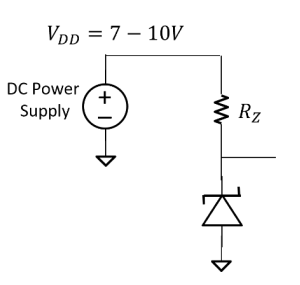
\includegraphics{./images/circuit1.png}}
\caption{Schematic with the Zener-based limiter assembled and validated during phase 1. \cite{week7}}
\label{circuit1}
\end{figure}

The bias direction of the diode was validated and the limiter was verified to produce a constant output equivalent to its Zener voltage. The diode was found to be biased in the right direction. However, the 4.3 V Zener diode was found to limit the voltage consistently to approximately 3.0 V, as shown in Table \ref{tab1}. This might be due to the temperature the diode was operating at. Since the Zener diode limited the voltage to a consistent value, the experiment was continued with a Zener voltage of 3.0 V.

\begin{table}[htbp]
\caption{Zener Diode $V_Z$ Measurements at Given $V_{DD}$ for Fig. \ref{circuit1}}
\begin{center}
\begin{tabular}{|p{\dimexpr0.5\linewidth-4\tabcolsep}|p{\dimexpr0.5\linewidth-4\tabcolsep}|}
\hline
\textbf{V\textsubscript{DD} (V)}&\textbf{V\textsubscript{z} (V)} \\
\hline
7.0 & 2.81 \\ \hline
7.5 & 2.85 \\ \hline
8.0 & 2.88 \\ \hline
8.5 & 2.91 \\ \hline
9.0 & 2.93 \\ \hline
9.5 & 2.96 \\ \hline
10.0 & 2.99 \\ \hline
\end{tabular}
\label{tab1}
\end{center}
\end{table}

\subsection{Testing the Linear Voltage Divider}

The second phase involved the assembly of the linear voltage divider, as depicted in Fig, by adding a 50 K$\Omega$ potentiometer. \ref{circuit2}. The potentiometer's resistance was adjusted until the voltage difference between the positive and negative terminal became close to zero when the supply voltage was set to the threshold voltage.

\begin{figure}[htbp]
\centerline{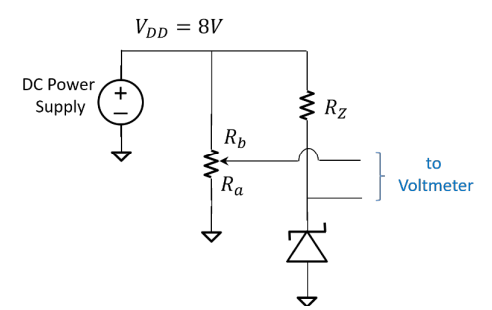
\includegraphics{./images/circuit2.png}}
\caption{Schematic with the linear voltage divider assembled and validated during phase 2. \cite{week7}}
\label{circuit2}
\end{figure}

\subsection{Testing the Voltage Comparator}

The third phase involved the assembly of the voltage comparator, as depicted in Fig \ref{circuit3}, by attaching a TLC3702 voltage comparator IC.

\begin{figure}[htp]
\centerline{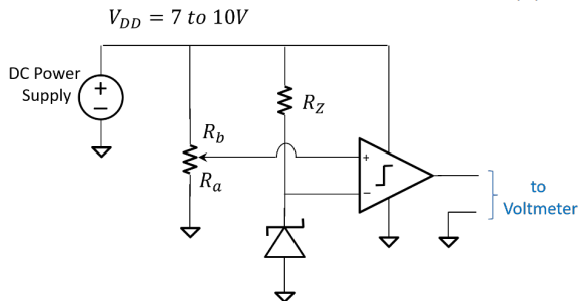
\includegraphics{./images/circuit3.png}}
\caption{Schematic with the linear voltage divider assembled and validated during phase 3. \cite{week7}}
\label{circuit3}
\end{figure}

The comparator was then verified to switches states at the threshold voltage. As depicted in Table \ref{tab2}, the output of the comparator is approximately $V_{SS}$, which is 0 V, when the value voltage supply reaches or is below the threshold value, which is 8 V. Also, the output of the comparator is approximately $V_{DD}$, which is approximately the value of the supply, when the value voltage supply is above the threshold value.

\begin{table}[htp]
\caption{Comparator $V_{out}$ Measurements at Given $V_{DD}$ for Fig. \ref{circuit4}}
\begin{center}
\begin{tabular}{|p{\dimexpr0.5\linewidth-4\tabcolsep}|p{\dimexpr0.5\linewidth-4\tabcolsep}|}
\hline
\textbf{V\textsubscript{DD} (V)}&\textbf{V\textsubscript{out} (v)} \\
\hline
7.0 & 0.00328 \\ \hline
7.5 & 0.000357 \\ \hline
8.0 & 0.000387 \\ \hline
8.5 & 8.499 \\ \hline
9.0 & 9.002 \\ \hline
9.5 & 9.501 \\ \hline
10.0 & 9.998 \\ \hline
\end{tabular}
\label{tab2}
\end{center}
\end{table}

\subsection{Testing the Optical Indicator}

The fourth phase involved the attachment of the LED and resistor, as depicted in Fig. \ref{circuit4}.
\begin{figure}[htbp]
\centerline{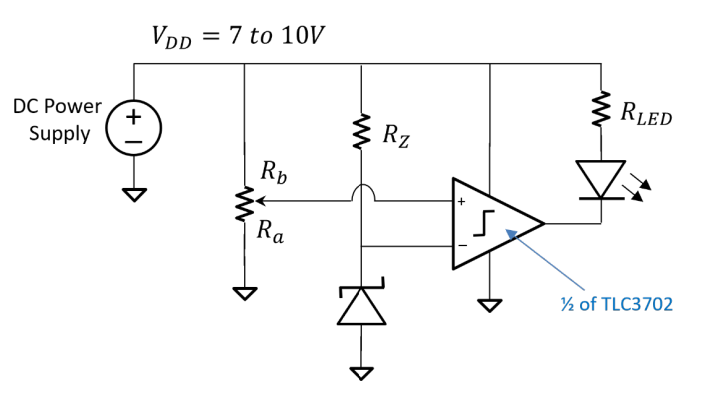
\includegraphics{./images/circuit4.png}}
\caption{Schematic with the optical indicator attached and validated during phase 4. \cite{week7}}
\label{circuit4}
\end{figure}

Since all of the components of the circuits were already rigorously tested in previous steps, this phase of the assembly was tested by simply observing whether the LED ignites when the supply voltage drops below the threshold voltage. The LED ignites when the supply voltage drops below the threshold voltage as depicted in Fig. \ref{circuitbuilt2}, and remains inactive when the supply voltage is above the threshold voltage as depicted in Fig. \ref{circuitbuilt1}

\begin{figure}[htbp]
\centerline{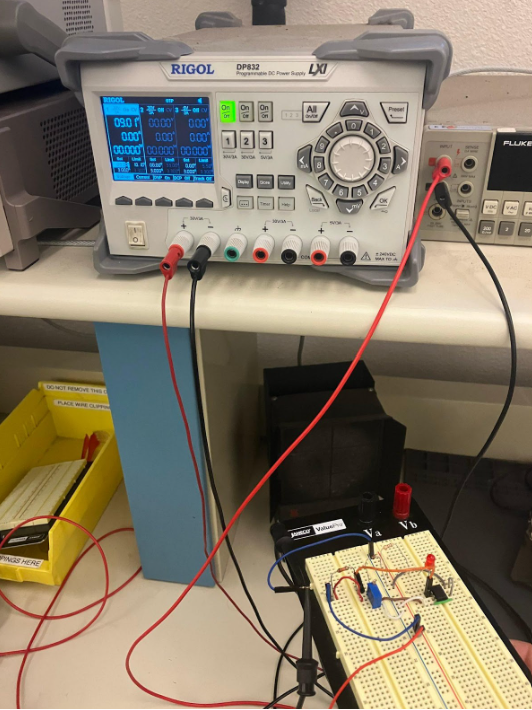
\includegraphics{./images/circuitbuilt1.png}}
\caption{Complete assembled circuit with indicator inactive when supply below the threshold voltage.}
\label{circuitbuilt1}
\end{figure}

\begin{figure}[htbp]
\centerline{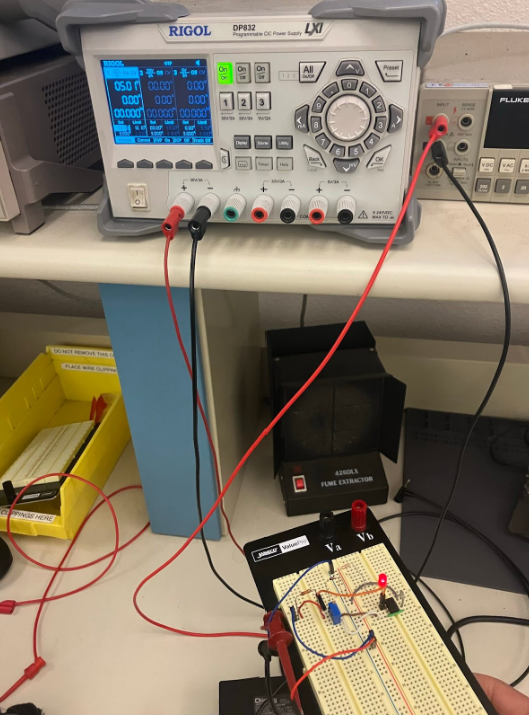
\includegraphics{./images/circuitbuilt2.png}}
\caption{Complete assembled circuit with indicator active when supply above the threshold voltage.}
\label{circuitbuilt2}
\end{figure}

\section{Conclusion}

This experiment demonstrated a functional and effective low-supply voltage sensor-indicator circuit and the successful assembly and operation of each phase of the circuit, emphasizing the importance of rigorous testing and analysis for reliable circuit performance. This also provided valuable insight into the performance characteristics and interactions of its individual components. The modular nature of the circuit design allows for flexibility in component selection and adaptation to specific application requirements.

\begin{thebibliography}{00}
\bibitem{week6} N. Ellis. (2023) "Week 6: Elementary Logic Circuits - Part II", Available https://canvas.calpoly.edu/courses/113173/files?preview=11616452
\bibitem{week7} N. Ellis. (2023) "Week 7: A Low-Supply Voltage Sensor with an Optical Indicator", Available \\https://canvas.calpoly.edu/courses/113173/files?preview=11699080
\bibitem{parts} N. Ellis. (2023) "EE145\_245\_parts.xlsx", Available \\ https://canvas.calpoly.edu/courses/113173/files?preview=10982615
\end{thebibliography}
\vspace{12pt}

\end{document}
